\documentclass[10pt,a4paper,makeidx]{book}

\usepackage[utf8x]{inputenc}
\usepackage{subfig}
\usepackage{amsmath,amsthm,amssymb,pifont,makeidx,geometry}
\usepackage{makeidx}
\usepackage{color}
\usepackage[pagebackref=true,breaklinks=true,colorlinks,bookmarks=false]{hyperref}
\usepackage{graphicx}
\usepackage{wasysym,pifont}
\definecolor{OliveGreen}{cmyk}{0.64,0,0.95,0.40}
\newcommand{\checkItem}{\textbf{\Pisymbol{wasy}{8}}\hspace{3mm}}
\newcommand{\command}[1]{\framebox[\textwidth][l]{\parbox[t]{\textwidth}{\tt \$ #1}}}
%\newcommand{\command}[1]{\framebox[\textwidth][l]{\tt \$ #1}}
\newcommand{\fileName}[1]{{\tt #1}}
\newcommand{\commandName}[1]{\textcolor{red}{\tt #1}}
\newcommand{\optionName}[1]{\textcolor{OliveGreen}{\tt #1}}
\newcommand{\outputName}[1]{\textcolor{blue}{\tt #1}}

\newcounter{thenote}
\newenvironment{note}{\stepcounter{thenote} \noindent \textcolor{red}{\textbf{Note \arabic{thenote}}~:}}{\par}
\newcommand{\warning}[1]{\textcolor{red}{\textbf{Warning~: #1}}}

\bibliographystyle{plain}

\graphicspath{{../images/}}
%\DeclareGraphicsRule{.jpg}{eps}{.ps.bb}{`convert #1 ps:-}
%\DeclareGraphicsRule{.gif}{eps}{.ps.bb}{`convert #1 ps:-}
%\DeclareGraphicsRule{.png}{eps}{.ps.bb}{`convert #1 ps:-}

\geometry{width=17cm,height=21.7cm}
\makeindex 

\title{{\textbf{\textcolor{blue}{OpenMEEG Tutorial\\
        {\Large EEG and MEG forward problems\\
                via the command-line interface.}}}}}
\author{Maureen Clerc\\Alexandre Gramfort \\
        Perrine Landreau\\Théo Papadopoulo}

\date{OpenMEEG Version 1.1\\2009}

\pdfpageattr {/Group << /S /Transparency /I true /CS /DeviceRGB>>}
\begin{document}

    \maketitle
    \tableofcontents

    \chapter{Context}
    \centerline{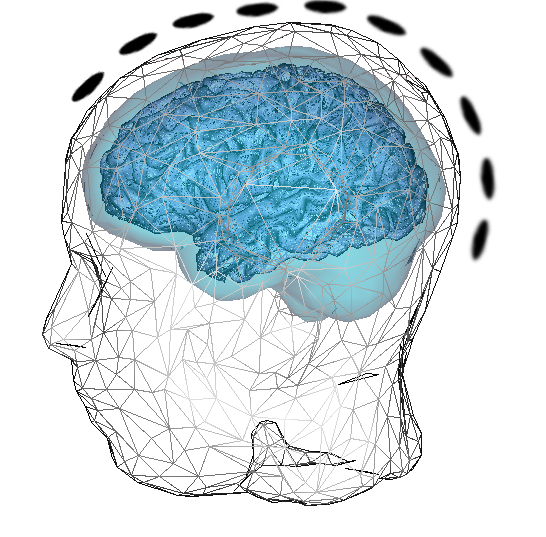
\includegraphics[height=9cm]{surf3.png}}

\noindent
The forward problem consists in simulating the electric potential (EEG) and magnetic fields (MEG) on the sensors due to electrical sources within the brain.

\centerline{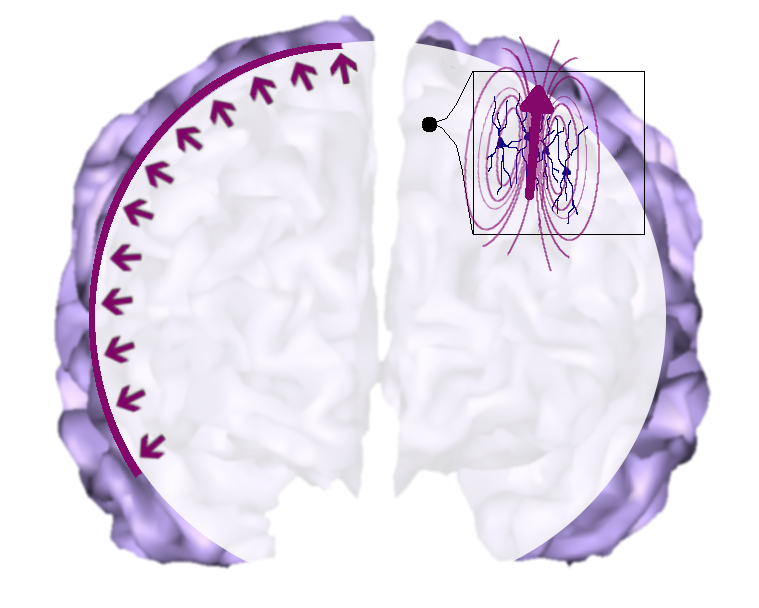
\includegraphics[height=10cm]{dipole.png}}

\noindent
\underline{Step 1}~: the potential is computed on \textbf{all surfaces } of the head model (scalp, outer skull and inner skull for a three-layer model).  Let $\mathbf{X}$ contain the values of the potential on the discretized surfaces, as well as the values of the normal current. The Boundary Element Method leads to a linear system:
\[
    \mathbf{HeadMat} . \mathbf{X} = \mathbf{SourceMat}
\]
See sections \ref{sect: command assemble HeadMat}, \ref{sect: command assemble SourceMat} and \ref{sect: command invert HeadMat}.

\medskip

\noindent
\underline{Step 2}~: the matrices relating the head model surfaces and the sensor data must be computed. These are different for EEG and for MEG.\\
\\
For EEG, the potential is interpolated from the surface discretization points to the sensor positions through a simple linear transformation~:\\
\[
    \left[ \mbox{potential at sensors} \right] =
    \left[ \mbox{interpolation matrix} \right] \times \left[ \mbox{potential at interfaces} \right] \mbox{in the case of EEG.}
\]
For MEG, the Biot and Savart equation allows to identify two contributions to the magnetic field: one which comes directly from the sources, and an ohmic contribution which comes from the volume conductor. 
Hence two linear transformations must be computed, one from the source locations  to MEG sensors, the other from the head model interfaces to the MEG sensors.\\

\noindent
See section \ref{sect: command assemble sensors}.

 
\medskip

\noindent
\underline{Step 3}~: the matrix relating the sources (at fixed positions and orientations) to the sensors is now ready to be computed (section \ref{sect: command gain}). This matrix is called  the \textbf{gain matrix} and is denoted  $\mathbf{G}$. The gain matrix is then applied to the source activation to simulate the forward problem  (section
\ref{sect: command direct}).


    \chapter{Data}
    \noindent
This chapter describes the type of data that is required to run a forward problem with OpenMEEG.
More detail on the data format is provided in Appendix~\ref{chap:format}.

\noindent
\underline{Meshes}~:\\
Meshes describing the interfaces between regions of homogeneous conductivity. These meshes generally represent:
\begin{itemize}
    \item the inner skull surface
    \item the outer skull surface
    \item the outer scalp surface
\end{itemize}

\noindent
The recommended mesh size is approximately 600 to 800 points per surface.


\medskip

\centerline{
    \hbox{\parbox[t]{5.5cm}{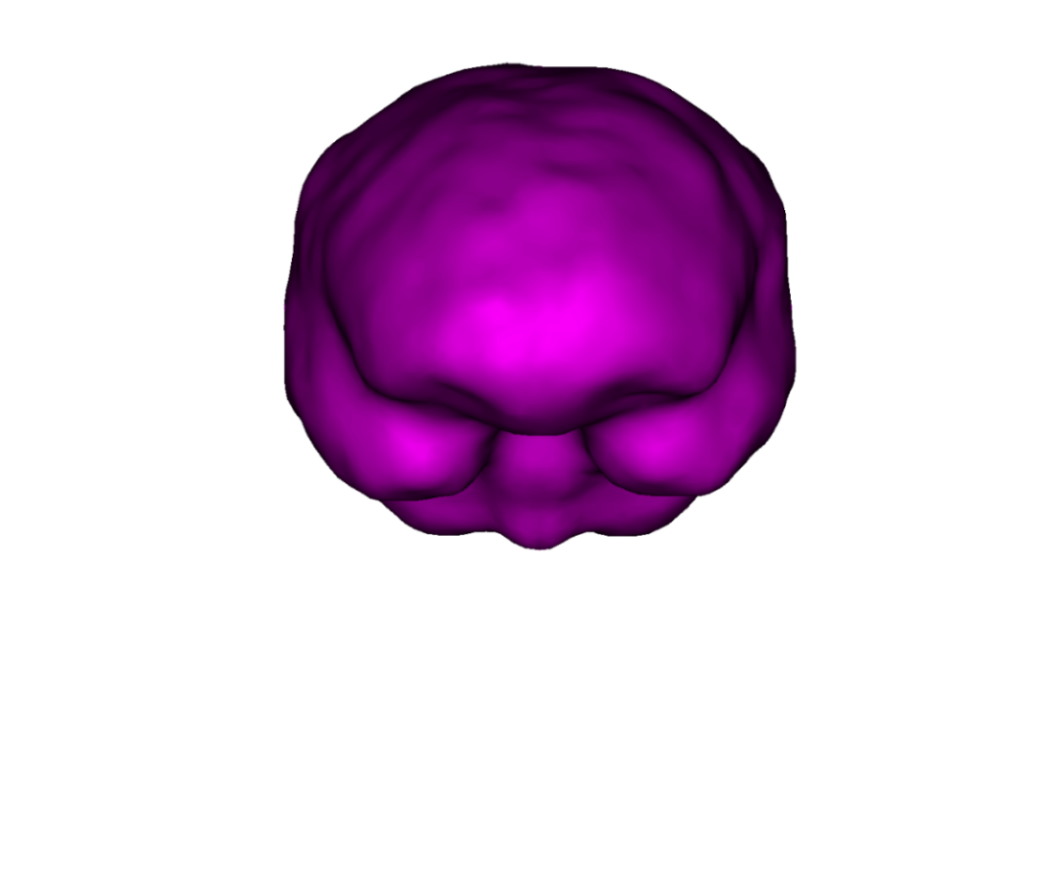
\includegraphics[width=5cm]{tete_couches_brain.png}\\
                            \parbox{5cm}{External surface of the cortex}}
          \parbox[t]{5.5cm}{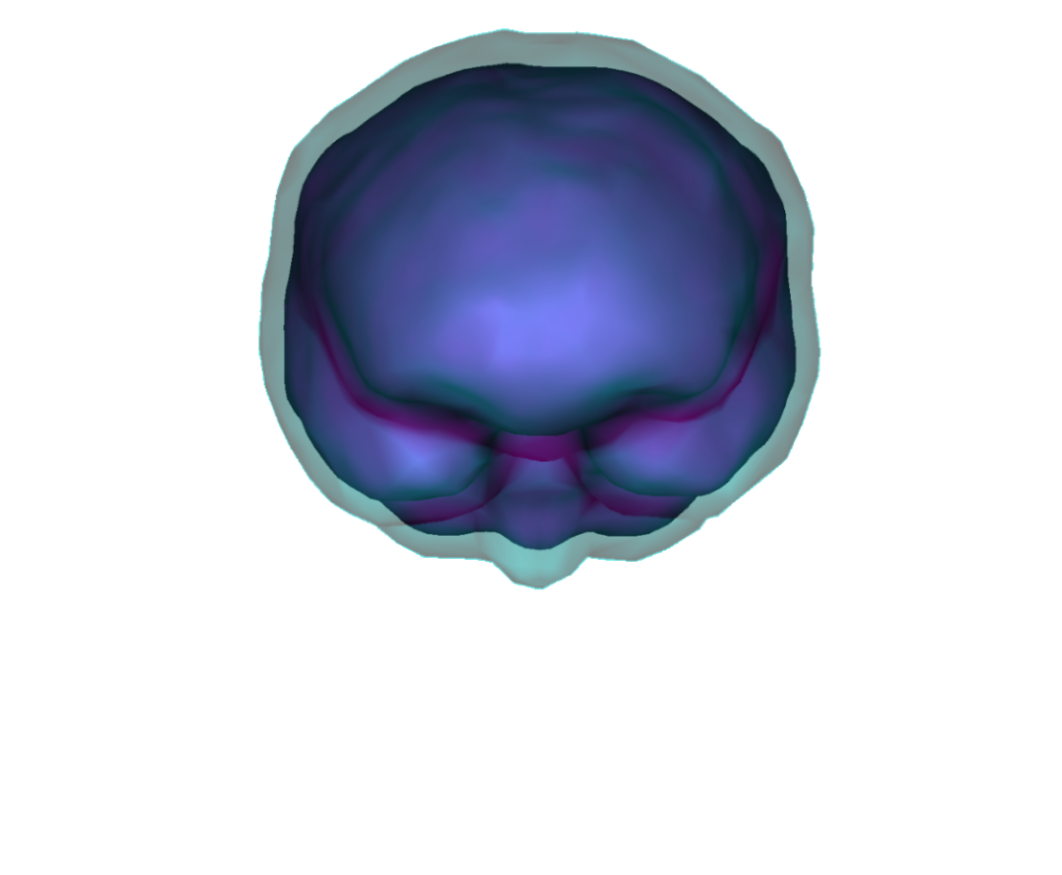
\includegraphics[width=5cm]{tete_couches_brainskull.png}\\\parbox{5cm}{External surface of the skull in blue and external surface of the cortex in fuchsia}}
          \parbox[t]{5.5cm}{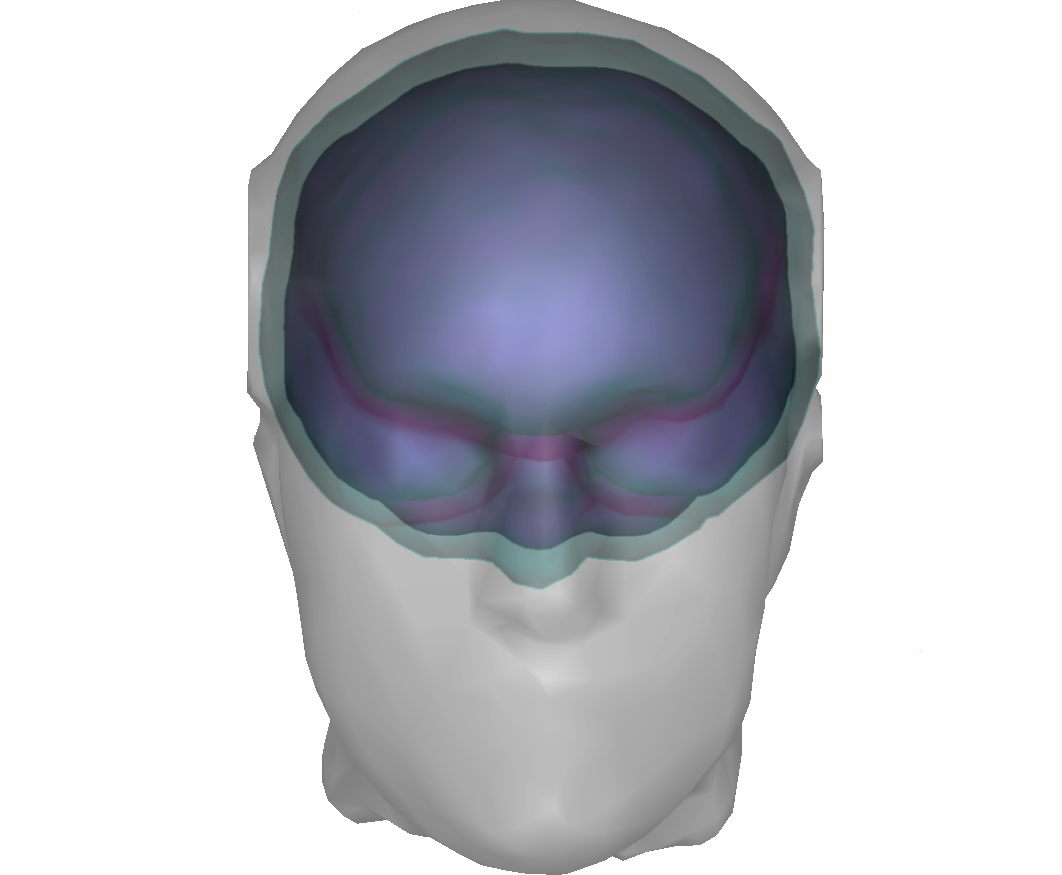
\includegraphics[width=5cm]{tete_couches_brainskullhead.png}\\
                            \parbox{5cm}{Example with three surfaces~:
                                  \begin{itemize}
                                       \item outer scalp (gray)
                                       \item outer skull (blue)
                                       \item inner skull (pink)
                                  \end{itemize}}
                            }
    }
}

\bigskip
\noindent
\underline{Sources}~:\\
Sources can be of two types: isolated or distributed. 
\noindent
For distributed sources, a source mesh describes their support. This is a detailed mesh generally covering the whole cortex. The mesh size should not exceed 35 000 points. 
The source amplitude is represented as continuous, and linear on each of the mesh triangles. The source orientation is modeled
as piecewise constant, normal to each of the mesh triangles.
\begin{center}
    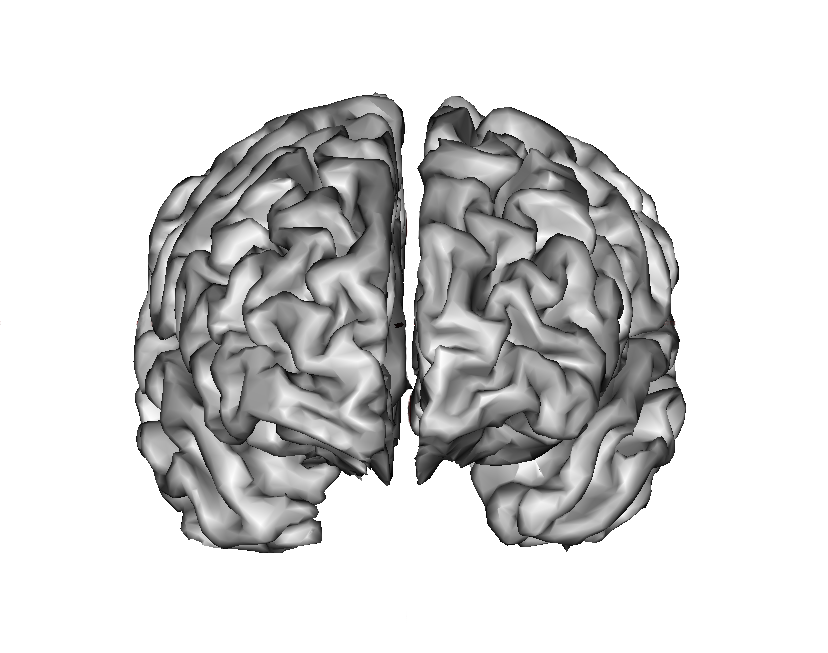
\includegraphics[height=9cm]{cortex.png}\\
Source mesh
\end{center}
\noindent
Isolated sources are the superposition of current dipoles, each of which is defined by its position and its moment.

\noindent
\underline{Sensors}~:
For EEG, the sensors are defined by the list of the x-y-z coordinates of the electrode positions. The electrodes are considered punctual and are called {\em patches}.	
The MEG sensor description is more complex, see  Appendix~\ref{chap:format}.


    \chapter{Commands}
    \noindent
In the following, the binaries in \commandName{red}, the options in \optionName{green}, the inputs are in  \textbf{black} and the outpus in  \outputName{blue}. 

\section{Head Matrix assembly $\mathbf{HeadMat}$:}
\label{sect: command assemble HeadMat}

\noindent
Inputs: 
\begin{itemize}
    \item \fileName{subject.geom}: geometry description file (see Appendix~\ref{sec:geom})
    \item \fileName{subject.cond}: conductivity description file (see Appendix~\ref{sec:cond})
\end{itemize}

\noindent
Output:
\begin{itemize}
    \item \outputName{HeadMat.bin}: binary file containing the matrix $\mathbf{HeadMat}$ (symmetric format).
\end{itemize}
The symmetric format only stores the lower half of a matrix.
\medskip

\noindent
\command{\commandName{om\_assemble} \optionName{-HeadMat} subject.geom subject.cond \outputName{HeadMat.bin}}
\medskip
Note: the abbreviated option names \optionName{-HM} or \optionName{-hm} can be used instead of \optionName{-HeadMat}.

\section{Source matrix assembly $\mathbf{Source}$:}
\label{sect: command assemble SourceMat}

\noindent
Inputs: 
\begin{itemize}
    \item \fileName{subject.geom}: geometry description file (see Appendix~\ref{sec:geom})
    \item \fileName{subject.cond}: conductivity description file (see Appendix~\ref{sec:cond})
    \item the source(s):
        \begin{description}
            \item [[dipolar case]] \fileName{dipolePosition.dip}: dipole description file (list of coordinates and orientations)
                                    (see Appendix~\ref{sec:dipoles}) 
            \item [[case of distributed sources]]  \fileName{sourcemesh}: source mesh (accepted formats:  *.tri or *.mesh of BrainVisa, or *.vtk) 
        \end{description}
\end{itemize}

\noindent
Output:
\begin{itemize}
    \item \outputName{SourceMat.bin}: binary file containing $\mathbf{SourceMat}$
\end{itemize}

\medskip

\noindent
For dipolar sources:\\
\noindent
\command{\commandName{om\_assemble} \optionName{-DipSourceMat} subject.geom subject.cond dipolePosition.dip \outputName{SourceMat.bin}}
\medskip
Note:  the abbreviated option names \optionName{-DSM} or \optionName{-dsm} can be used instead of \optionName{-DipSourceMat}.

\medskip

\noindent
For distributed sources:\\
\noindent
\command{\commandName{om\_assemble} \optionName{-SurfSourceMat} subject.geom subject.cond sourcemesh \outputName{SourceMat.bin}}
\medskip
Note: the abbreviated option names  \optionName{-SSM} or \optionName{-ssm}  can be used instead of  \optionName{-SurfSourceMat}.

\section{$\mathbf{HeadMat}$ matrix inversion:}
\label{sect: command invert HeadMat}

\noindent
Inputs:
\begin{itemize}
    \item \fileName{HeadMat.bin}: binary file containing matrix $\mathbf{HeadMat}$ (symmetric format)
\end{itemize}

\noindent
Output:
\begin{itemize}
    \item \outputName{HeadMatInv.bin}: binary file containing matrix $\mathbf{HeadMat}^{-1}$ (symmetric format)
\end{itemize}

\medskip

\noindent
\command{\commandName{om\_minverser} HeadMat.bin \outputName{HeadMatInv.bin}}

\section{Linear transformation from X to the sensor potential:}
\label{sect: command assemble sensors}

\checkItem \underline{For EEG}:\\

A linear interpolation is computed which relates X to the electrode potential through the linear transformation:
\[
    \mathbf{V_{electrode}} = \mathbf{Head2EEG} . \mathbf{X}
\]
where:
\begin{itemize}
    \item $\mathbf{V_{electrode}}$ is the column-vector of potential values at the sensors (output of EEG forward problem),
    \item $\mathbf{X}$ is the column-vector containing the values of the potential and the normal current on all the surface of the model,
    \item $\mathbf{Head2EEGMat}$ is the linear transformation to be computed.
\end{itemize}

\bigskip

\noindent
Inputs:
\begin{itemize}
    \item \fileName{subject.geom}: geometry description file (see Appendix~\ref{sec:geom})
    \item \fileName{subject.cond}: conductivity description file (see Appendix~\ref{sec:cond})
    \item \fileName{patchespositions.txt}: file containing the positions of the EEG electrodes (see Appendix~\ref{sec:sensors})
\end{itemize}
Sortie:
\begin{itemize}
    \item \outputName{Head2EEGMat.bin}: file containing the matrix $\mathbf{Head2EEGMat}$ (sparse format)
\end{itemize}
The sparse format allows to store efficiently matrices containing a small proportion of non-zero values.
\medskip

\noindent
\command{\commandName{om\_assemble} \optionName{-Head2EEGMat} subject.geom subject.cond patchespositions.txt \outputName{Head2EEGMat.bin}}
\medskip
Note: the abbreviated option names \optionName{-H2EM} or \optionName{-h2em} can be used instead of \optionName{-Head2EEGMat}.

\bigskip

\checkItem \underline{For MEG}:\\
In the case of MEG there are more matrices to assemble, as explained in section~\ref{}. The magnetic field is related both to the sources directly, as well as to the electric  potential, according to:
\[
    \mathbf{M_{sensor}} = \mathbf{Source2MEGMat} . \mathbf{S} + \mathbf{Head2MEGMat}.\mathbf{X}
\]

\medskip

\noindent
\underline{Contribution to MEG from the potential ($\mathbf{Head2MEGMat}$)}:\\
Inputs:
\begin{itemize}
    \item \fileName{subject.geom}: geometry description file (see Appendix~\ref{sec:geom})
    \item \fileName{subject.cond}: conductivity description file (see Appendix~\ref{sec:cond})
    \item \fileName{sensorpositions.txt}: positions and orientations of MEG sensors (see Appendix~\ref{sec:sensors})
\end{itemize}
Output:
\begin{itemize}
    \item \outputName{Head2MegMat.bin}: binary file containing $\mathbf{Head2MEGMat}$
\end{itemize}

\medskip

\noindent
\command{\commandName{om\_assemble} \optionName{-Head2MEGMat} subject.geom subject.cond sensorpositions.txt \outputName{Head2MEGMat.bin}}
\medskip
Note:  the abbreviated option names \optionName{-H2MM} or \optionName{-h2mm} can be used instead of \optionName{-Head2MEGMat}.

\bigskip

\noindent
\underline{Contribution to MEG from the sources ($\mathbf{Source2MEGMat}$)}:\\
Inputs:
\begin{itemize}
    \item the source(s):
    \begin{description}
        \item [[dipolar sources]] \fileName{dipolePosition.dip}:  dipole description file (list of coordinates and orientations) (see Appendix~\ref{sec:dipoles}) 
        \item [[distributed sources]] \fileName{sourcemesh}:  source mesh (accepted formats:  *.tri or *.mesh of BrainVisa, or *.vtk) 
    \end{description}
    \item \fileName{sensorpositions.txt}: positions and orientations of MEG sensors (see Appendix~\ref{sec:sensors})
\end{itemize}
Output: 
\begin{itemize}
    \item \outputName{DipSource2MEGMat.bin}: binary file containing $\mathbf{DipSource2MEGMat}$ \\
\item or \outputName{SurfSource2MEGMat.bin}: binary file containing $\mathbf{SurfSource2MEGMat}$ 
\end{itemize}

\medskip

\noindent
For dipolar sources:\\
\noindent
\command{\commandName{om\_assemble} \optionName{-DipSource2MEGMat} dipolePosition.dip sensorpositions.txt \outputName{DipSource2MEGMat.bin}}
\medskip
Note:  the abbreviated option names \optionName{-DS2MM} or \optionName{-ds2mm} can be used instead of \optionName{-DipSource2MEGMat}.

\medskip

\noindent
For distributed sources:\\
\noindent
\command{\commandName{om\_assemble} \optionName{-SurfSource2MEGMat} sourcemesh sensorpositions.txt \outputName{SurfSource2MEGMat.bin}}
\medskip
Note:   the abbreviated option names  \optionName{-SS2MM} or \optionName{-ss2mm} can be used instead of \optionName{-SurfSource2MEGMat}.

\section{Gain matrix computation:}
\label{sect: command gain}

The gain matrix represents the linear transformation relating the activation of sources, at \textbf{predefined positions and orientations} to the values of the fields of interest (electric potential or magnetic field) at predefined sensor positions (and orientations for MEG). 

\checkItem \underline{For EEG}:\\
Inputs:
\begin{itemize}
    \item \fileName{HeadMatInv.bin}: binary file containing $\mathbf{HeadMat}^{-1}$ (symmetric format)
    \item \fileName{SourceMat.bin}: binary file containing either  $\mathbf{SurfSourceMat}$ or  $\mathbf{DipSourceMat}$
    \item \fileName{Head2EEGMat.bin}: binary file containing $\mathbf{Head2EEGMat}$ (sparse format)
\end{itemize}
Output:
\begin{itemize}
    \item \outputName{GainEEGMat.bin}: binary file contining the gain matrix
\end{itemize}

\medskip

\noindent
\command{\commandName{om\_gain} \optionName{-EEG} HeadMatInv.bin SourceMat.bin Head2EEGMat.bin \outputName{GainEEGMat.bin}}


\bigskip

\checkItem\underline{For MEG}:\\
Inputs:
\begin{itemize}
    \item \fileName{HeadMatInv.bin}: binary file containing $\mathbf{HeadMat}^{-1}$ (symmetric format)
    \item \fileName{SourceMat.bin}: binary file containing either  $\mathbf{SurfSourceMat}$ or  $\mathbf{DipSourceMat}$
    \item \fileName{Head2MEGMat.bin}: binary file containing $\mathbf{Head2MEGMat}$
    \item \fileName{Source2MEGMat.bin}:binary file containing either  $\mathbf{DipSource2MEGMat}$ or $\mathbf{SurfSource2MEGMat}$
\end{itemize}
Output:
\begin{itemize}
    \item \outputName{GainMEGMat.bin}: binary file containing the gain matrix
\end{itemize}

\medskip

\noindent
\command{\commandName{om\_gain} \optionName{-MEG} HeadMatInv.bin SourceMat.bin Head2MEGMat.bin Source2MEGMat.bin \outputName{GainMEGMat.bin}}


\section{The forward problem:}
\label{sect: command direct}

Once the gain matrix is computed, the forward problem amounts to defining the source activation, and applying the gain matrix to this activation.

Inputs: 
\begin{itemize}
    \item \fileName{GainMat.bin}: binary file containing EEG or MEG gain matrix
    \item \fileName{activationSources.txt}: file describing the source activation (see Appendix~\ref{sec:activ})
    \item \fileName{noise}: noise (zero, or positive real number)
\end{itemize}
Output:
\begin{itemize}
    \item \outputName{sensorResults.txt}: file containing the simulated sensor data.
\end{itemize}

\medskip

\noindent
\command{\commandName{om\_forward} gainMat.bin activationSources.txt \outputName{sensorResults.txt} noise}


    \appendix
    \chapter{Data format}
	\label{chap:format}
    \section{Geometry description file}
\label{sect: annexe 1}
{\huge TO BE TRANSLATED}\\
\noindent
Ce fichier décrit la géométrie utilisée~: le nombre et le nom des surfaces maillées séparant les différents domaines de
conductivité ainsi que le nombre et le nom de chacun de ces domaines et leur disposition par rapport aux surfaces précédemment
citées.\\ 
Extension du fichier~: *.geom par convention. 

\centerline{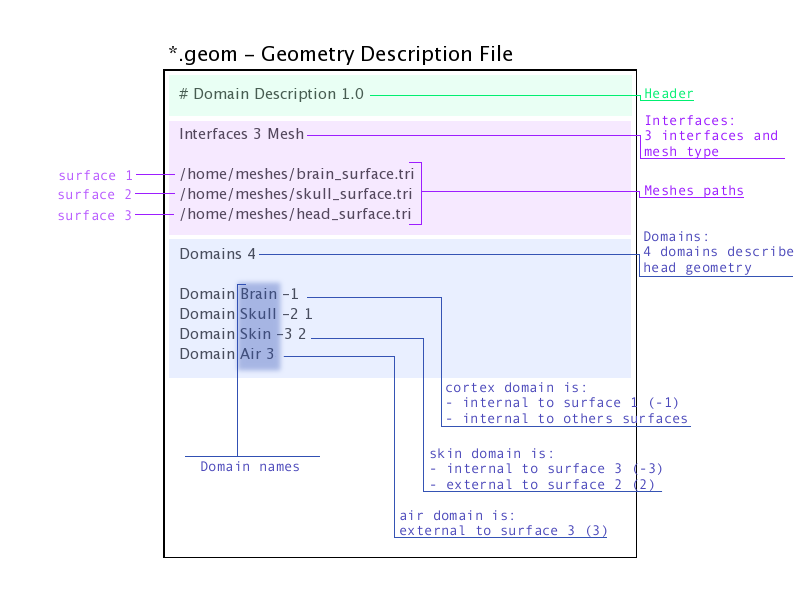
\includegraphics[height=9cm]{geom.png}}

\begin{note}
    nous avons un bug qui peut survenir sur l'ordre des domaines. Il est alors préférable de noter les domaines de la manière
    suivante (noter en premier la référence aux surfaces externes et en deuxième position la surface interne)~:

    \begin{tabular}{ll}
        Domain Brain -1              & \\
        Domain Skull \textbf{1 -2}	 &	\emph{au lieu de Domain Skull -2 1} \\
        Domain Skin \textbf{2 -3}	 &	\emph{au lieu de Domain Skin -3 2}  \\
        Domain Air 3                 &  \\
    \end{tabular}
\end{note}

\medskip

\begin{note}
    les "Meshes paths" sont 
    \begin{itemize}
        \item soit absolus (comme le montre le dessin)
        \item soit relatifs à l'endroit où on exécute les lignes de commandes 
    \end{itemize}
    Seuls les formats suivants sont lus pour les surfaces maillées~:
    \begin{itemize}
        \item *.tri~: format TRI issu des premières versions de BrainVisa. Aussi lu par Anatomist.
        \item *.mesh~: format MESH issu des versions 3.0.2 et plus de BrainVisa. Aussi lu par Anatomist.
        \item *.vtk~: format de maillage VTK.
    \end{itemize}
\end{note}


\section{Fichier de description des conductivités}
\label{sect: annexe 2}

\noindent
Ce fichier décrit les valeurs des conductivités associées aux différents domaines déclarés dans le fichier de description de la
géométrie.\\ 
Extension du fichier~: *.cond par convention.\\
\warning{Attention~:  bien respecter la casse entre les noms de domaines donnés dans le fichier de description de la géométrie et ceux
notés dans le fichier de description des conductivités !}

\centerline{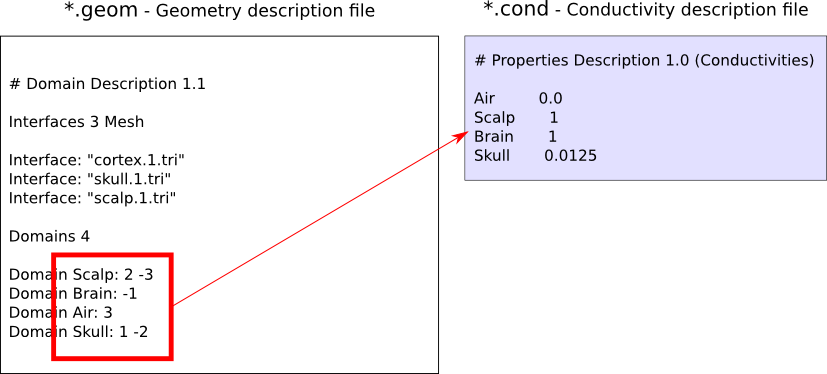
\includegraphics[height=9cm]{cond.png}}

\begin{note}
    ce sont des conductivités relatives~: l'air n'est pas conducteur, donc a une conductivité nulle, le cerveau est considéré
    comme étant entièrement conducteur tout comme la peau et le crâne a une conductivité égale à 1/80 de celle du cerveau.
\end{note}

\section{Position et orientation des dipôles}
\label{sect: annexe 3}

\noindent
Fichier texte. A une ligne donnée correspond un dipôle~: 
\begin{itemize}
    \item les trois premiers nombres (séparés par un espace) sont les coordonnées cartésiennes de la position du dipôle,
    \item les trois derniers nombres (séparés par un espace) sont les coordonnées cartésiennes du vecteur normale donnant
           l'orientation du dipôle.
\end{itemize}
Extension de fichier~: *.dip ou *.txt.

\medskip

\noindent
Dans l'exemple ci dessous, sont décrits 5 dipôles~:

\centerline{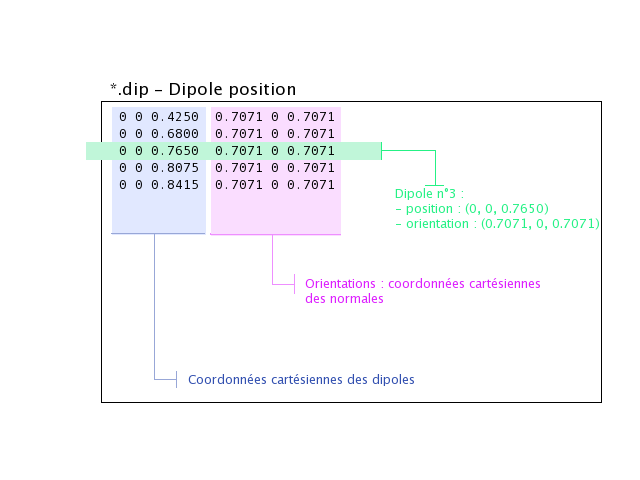
\includegraphics[height=9cm]{dipolePositions.png}}

\begin{note}
    les coordonnées sont prises dans le même repère que celui des maillages (repère de l'IRM en général)
\end{note}

\section{Position (et orientation) des capteurs}
\label{sect: annexe 4}

\noindent
Dans le cas de l'EEG, il s'agit d'un fichier de description de la position des capteurs en coordonnées cartésiennes et dans le
même repère que celui des maillages (en général, le repère de l'IRM). A une ligne correspond les coordonnées d'un capteur
séparées par un espace. 

\medskip

\noindent
Dans le cas de la MEG, il s'agit d'un fichier de description de la position et de l'orientation des capteurs en coordonnées
cartésiennes et dans le même repère que celui des maillages (en général, le repère de l'IRM). A une ligne correspond les
coordonnées d'un capteur (séparées par un espace) suivies des coordonnées du vecteur orientation normé (séparés par un espace).

\section{Activation des sources}
\label{sect: annexe 5}

\noindent
Les fichiers d'activation des sources sont des fichiers texte. A une ligne correspond une source~: 
\begin{itemize}
    \item dans le cas dipolaire, sont écrits sur la ième ligne les états d'activation du ième dipôle,
    \item dans le cas des sources distribuées, sont écrits sur la ième ligne les états d'activation du ième point du maillage
          des sources.
\end{itemize}

\medskip

\noindent
On trouve en colonne les temps auxquels sont associés les activations.

\medskip

\noindent
Exemple dans le cas dipolaire~:

\centerline{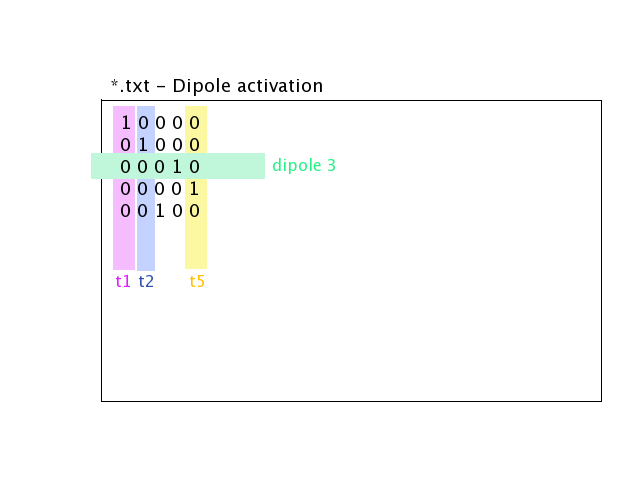
\includegraphics[height=9cm]{dipActiv.png}}


\end{document}
